\documentclass{hbrs-ecta-report}

\usepackage{float}
\usepackage{placeins}
\usepackage{german}
\begin{document}

\conferenceinfo{H-BRS}{2017}

\title{Neuroevolution: Simple Hill Climbing}
\subtitle{}

\numberofauthors{2}
\author{
\alignauthor
Tim L"ugger, Jan Urfei
}

\date{today}
\maketitle
\begin{abstract}
Aufgabe: Implementiere den HillClimb Algorithmus aus der Vorlesung und f"uhre diesen 100 Mal mit einer vorgegebenen Kostenfunktion aus.
\end{abstract}

%% ------------------------------ GENERAL NOTES ------------------------------ %%
\section{General Notes}

%% ------------------------------ REPORT STRUCTURE ------------------------------ %%

\subsection{Der HillClimb Algorithmus}
Der HillClimb Algorithmus ben"otigt eine Kostenfunktion, anhand derer er das Ergebnis bewerten kann, um die optimale L"osung zu finden. Zu erst wird sich ein zuf"alliger Punkt ausgesucht und von diesem werden die Kosten mittels der Kostenfunktion berechnet. Als n"achstes werden benachbarte Punkte gesucht und von diesen und dem alten Punkt werden die Kosten bestimmt. Von all diesen Punkten wird das Maximum bestimmt. Dieser Punkt wird als neuer Punkt genommen von dem neue Nachbarn gebildet werden. Der Algorithmus endet entweder nach einer festen Anzahl an Iterationen oder wenn sich das Ergebnis nicht mehr "andert.

\subsection{Verbesserung}

\section{Unser Experiment}
\subsection{Unsere Kostenfunktion}
\begin{figure}[ht!]
\centering
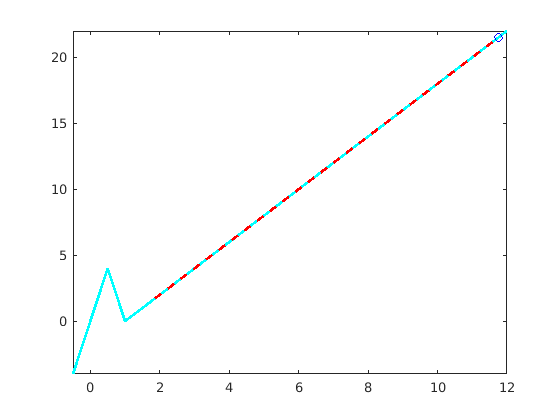
\includegraphics[width=\linewidth]{img/plot_fit_max.png}
\caption{Development of average mean square error, comparing NEAT and ESP}
\label{fig:1} 
\end{figure}
\subsection{Unsere Ergebnisse}



\FloatBarrier
\section{Conclusion}


\newpage


\bibliographystyle{abbrv}
\bibliography{HeteroNEAT} 
\end{document}
}